\chapter{Тестирование и анализ полученной модели}
\label{sec:analysis}

В данной главе приводится описание метода тестирования полученного инструмента для работы с данными.

Для тестирования использовался подход модульного тестирования. Причины данного выбора:

\begin{itemize}
  \item проверка корректности работы операций и функций библиотеки;
  \item подготовка к последующим оптимизациям алгоритмов;
  \item подготовка примеров использования разработанных методов в реальной ситуации.
\end{itemize}

Идея состоит в том, чтобы писать тесты для каждой реализованной операции.
Это позволяет достаточно быстро проверить, не привело ли очередное изменение кода к регрессии,
то есть к появлению ошибок в уже оттестированных местах программы,
а также облегчает обнаружение и устранение таких ошибок. Конечный пользователь данного продукта,
может использовать эти тесты как примеры. В качестве эталона в тестах,
использовались операции и функции LINQ, где это было возможно.

В ходе тестирования важно было проверить два свойства реализованных структур данных:

\begin{itemize}
  \item корректность применение операции;
  \item корректно сгенерированные события изменения данных.
\end{itemize}

Корректность применения операции проверялся сравнением результата выполнения операции с эталоном,
события --- с помощью специальных обработчиков, которые определяли тип сгенерированного изменения.

Тесты сгруппированы по операциям и протестированы все возможные методы и события
для реализованных структур данных в данном проекте. Стандартный тест для операции включает в себя:

\begin{itemize}
  \item инициализация исходных данных;
  \item применение операции к данным;
  \item применение эталонной операции к данным;
  \item функция тестирования свойства(добавление, удаление и т. д.);
  \item пуск теста с сгенерированными данными.
\end{itemize}

\begin{lstlisting}[style=csharpinlinestyle, caption={Пример теста}, label=lst:analysis:test]
[TestMethod]
public void UpdateItem()
{
  \\ initialization
  IObservableCollection<BehaviorSubject<int>> collection = new ObservableCollection<BehaviorSubject<int>>();

  \\ create actual data
  IObservableReadOnlyCollection<int> actualOperation = collection
    .WhereRc(_filter, _getUpdater)
    .SelectRc(_selector, _getUpdater);

  \\ create expected data
  IEnumerable<int> expectedOperation = collection.Where(_filter).Select(_selector);

  \\test function body
  Action<BehaviorSubject<int>> assertAddAndUpdate = item =>
  {
    collection.Add(item);
    Assert.IsTrue(Enumerable.SequenceEqual(expectedOperation, actualOperation));
    item.OnNext(item.Value + 1);
    Assert.IsTrue(Enumerable.SequenceEqual(expectedOperation, actualOperation));
    item.OnNext(item.Value + 1);
    Assert.IsTrue(Enumerable.SequenceEqual(expectedOperation, actualOperation));
  };

  \\start test
  Prop.ForAll(Arb.From(_intGen), assertAddAndUpdate).QuickCheckThrowOnFailure();
}
\end{lstlisting}

В листинге~\ref{lst:analysis:test} приведен пример одного теста на изменение обекта в коллекции. Данный тест проверят
как применяется операция и правильные ли генерирует события. В качестве платформы тестирования использовался Unit Test Framework,
который поставляется вместе с Visual Studio. Для генерации тестовых данных используется библиотека FsCheck, написанная на языке \fsharp{}.
Она предназначена для реализации модульного и функционального тестирования программных систем. Уже на примере теста видно, как мало требуется написать кода, чтобы создать коллекцию реагирующую на изменения исходных данных.

\begin{figure}[ht]
\centering
  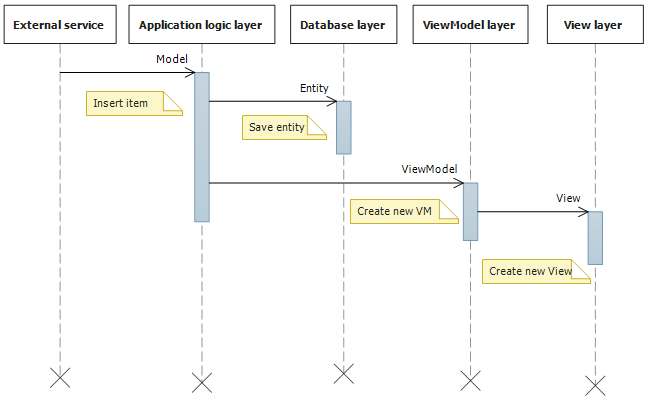
\includegraphics[scale=0.7]{mvvm_example.png}
  \caption{ Использование с паттерном MVVM }
  \label{fig:mvvm_example}
\end{figure}

Рассмотрим пример использования данной библиотеки вместе с паттерном проектирования MVVM(Model-View-ViewModel)~\cite{mvvm_pattern}. На рисунке~\ref{fig:mvvm_example} представлено:

\begin{itemize}
  \item External service layer --- внешний сервис, который предоставил новую модель;
  \item Application logic layer --- бизнес логика приложения;
  \item Database layer --- слой доступа к базе данных;
  \item ViewModel layer --- слой абстракций для моделей и представлений;
  \item View layer --- слой пользовательского интерфейса.
\end{itemize}

По сценарию в систему приходит новая модель. Нам требуется сохранить её в базу данных, создать из нее ViewModel, а из ViewModel --- View. А данном случае, Application logic layer будет содержать объект наблюдаемой коллекции, на который будут подписаны Database layer и ViewModel layer. При добавлении элемента в коллекцию, изменения распространятся автоматически на всю систему. Для реализации данного примера достаточно операции Select(проекции) и операции Dispatch(перенаправления в другой поток исполнения).

Так добавив по несколько строк кода в каждый уровень приложения, можно создать связь между пользовательским интерфейсом и бизнес-логикой, используя только операции данной библиотеки. Используя понятия реляционной алгебры, код получается легко читаемым для широкого круга разработчиков.
